\chapter{Experiments and Results}
\label{c:experiments_and_results}

To verify the claimed properties of FileFarm, we conduct a series of experiments. In this chapter, we will describe our experimental environment first, and then describe settings, process, and results of each experiments.

% Environment
\section{Environment}
\label{s:expenvironment}

In the following experiments, we run FileFarm on 10 physical hosts with following system information:

\begin{itemize}
    \item CPU: Intel(R) Xeon(R) CPU E5-1630 v3 @ 3.70GHz
    \item Memory: 16 GiB DDR4
    \item Network Interface: Ethernet Connection (2) I218-LM (1Gbit/s)
    \item Operating System: Ubuntu Server 18.04.2 LTS
\end{itemize}

 \noindent Each of the 10 physical hosts is assigned with a static IP address, and all of the 10 IP addresses belong to the same subnet with mask 255.255.255.0. Depending on settings of each experiment, a physical host might runs one or multiple instances of FileFarm farmers and clients simultaneously.

% exp: NODE_LOOKUP Efficiency
\section{Experiment: NODE\_LOOKUP Efficiency}
\label{s:expnodelookupefficiency}

In FileFarm, each shard is stored on exactly $K$ farmers. Instead of saving location of shards as static records in a centralized database, FileFarm adopts Kademlia's dynamical lookup procedures. Thus, the efficiency of these procedures will impact system's I/O performance greatly. According to the sketch of proof in \cite{maymounkov2002kademlia}, NODE\_LOOKUPs in a Kademlia network will finish in $\lceil log(n) \rceil + c$ steps for some small constant of $c$, where $n$ is network size, i.e., number of nodes in the network. We want to verify that this property also holds in FileFarm.

In this experiment, we first start $n$ farmers. After all farmers are bootstrapped, we make each farmer perform NODE\_LOOKUP on 100 random targets and report the number of steps needed to locate the $K$ closest farmers around the target. Then we collect and compute mean of steps needed. The whole process is repeated for $n=1,10,20,30,40,50,60,$ $70,80,90,100,110,120,130,140,150$ and $K=1,2,3,4,5$.

\begin{figure}[hbt]
\centering
  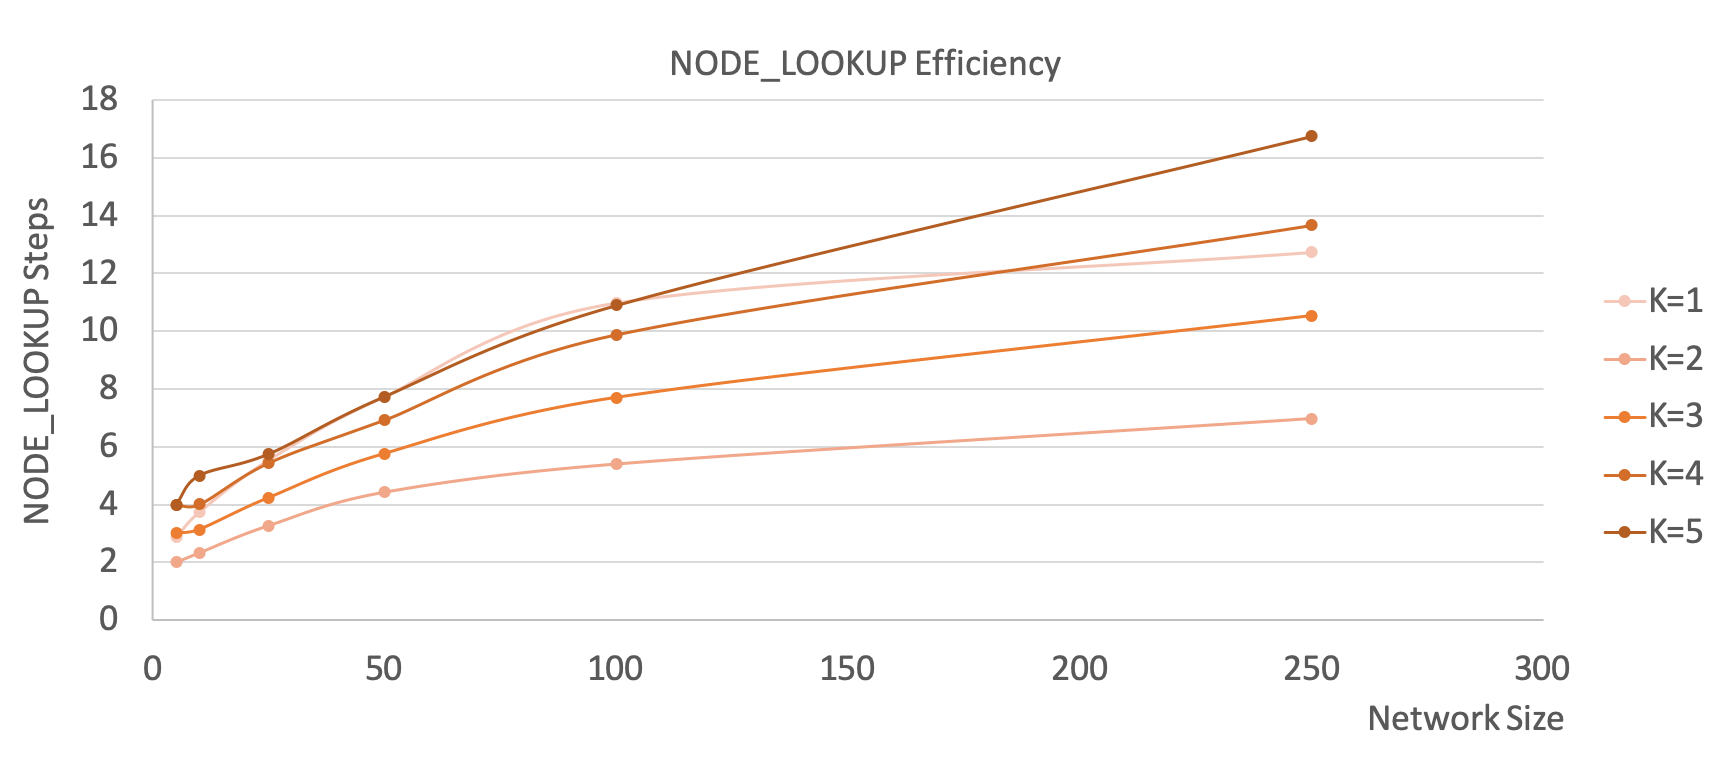
\includegraphics[width=14cm]{charts/chart_node_lookup_efficiency.png}
  \caption[NODE\_LOOKUP steps with respect to $K$ and network size $n$]{NODE\_LOOKUP steps with respect to redundancy parameter $K$ and network size $n$. The curve shows a logarithm relationship between NODE\_LOOKUP steps and network size.}
  \label{fig:nodelookupefficiency}
\end{figure}

From Figure \ref{fig:nodelookupefficiency}, we can observe that number of NODE\_LOOKUP steps grows with number of farmers, following a logarithm-like curve. With number of farmers growing from 50 to 100, it only takes around 2 more steps to locate all $K$ closest farmers, which makes FileFarm network scalable. However, it can also be observed that a larger setting of $K$ requires more steps for NODE\_LOOKUP procedure to finish, which is intuitive, considering the fact that NODE\_LOOKUP finds all of the $K$ closest farmers, instead of one or some of them.


% exp: VALUE_LOOKUP Efficiency
\section{Experiment: VALUE\_LOOKUP Efficiency}
\label{s:expvaluelookupefficiency}

Just like performing NODE\_LOOKUP before uploading a shard, farmers perform VALUE\_LOOKUP before downloading a shard. Different from NODE\_LOOKUP, the VALUE\_LOOKUP procedure finishes immediately when the target value is found. Thus, VALUE\_LOOKUP procedure only needs to reach any one of the $K$ closest farmers instead of finding all of them. According to Cai's analysis\cite{cai2013probabilistic}, it takes no more than $(1+O(1))\frac{log(n)}{H_{K}}$ steps for any node in a Kademlia network to locate any other node, where $H_K = \sum_{i=1}^{K} 1/i$. This upper bound also stands for VALUE\_LOOKUP, considering the fact that VALUE\_LOOKUP for the target key converges along the same path as NODE\_LOOKUP for the closest farmer, due to $unidirectionality$ of XOR distance metric. In this experiment, we want to verify this property on FileFarm and compare the result with \ref{s:expnodelookupefficiency}.

In this experiment, we first start $n$ farmers. After all farmers are bootstrapped, we starts 10 clients and make them upload 50 random files in total. Then we make clients send file download requests randomly and let farmers report the number of steps needed for each VALUE\_LOOKUP. We collect around 500 VALUE\_LOOKUP records and compute mean of steps needed. The whole process is repeated for  $n=1,10,20,30,40,50,60,70,80,90,$ $100,110,120,130,140,150$ and $K=1,2,3,4,5$.

\begin{figure}[hbt]
\centering
  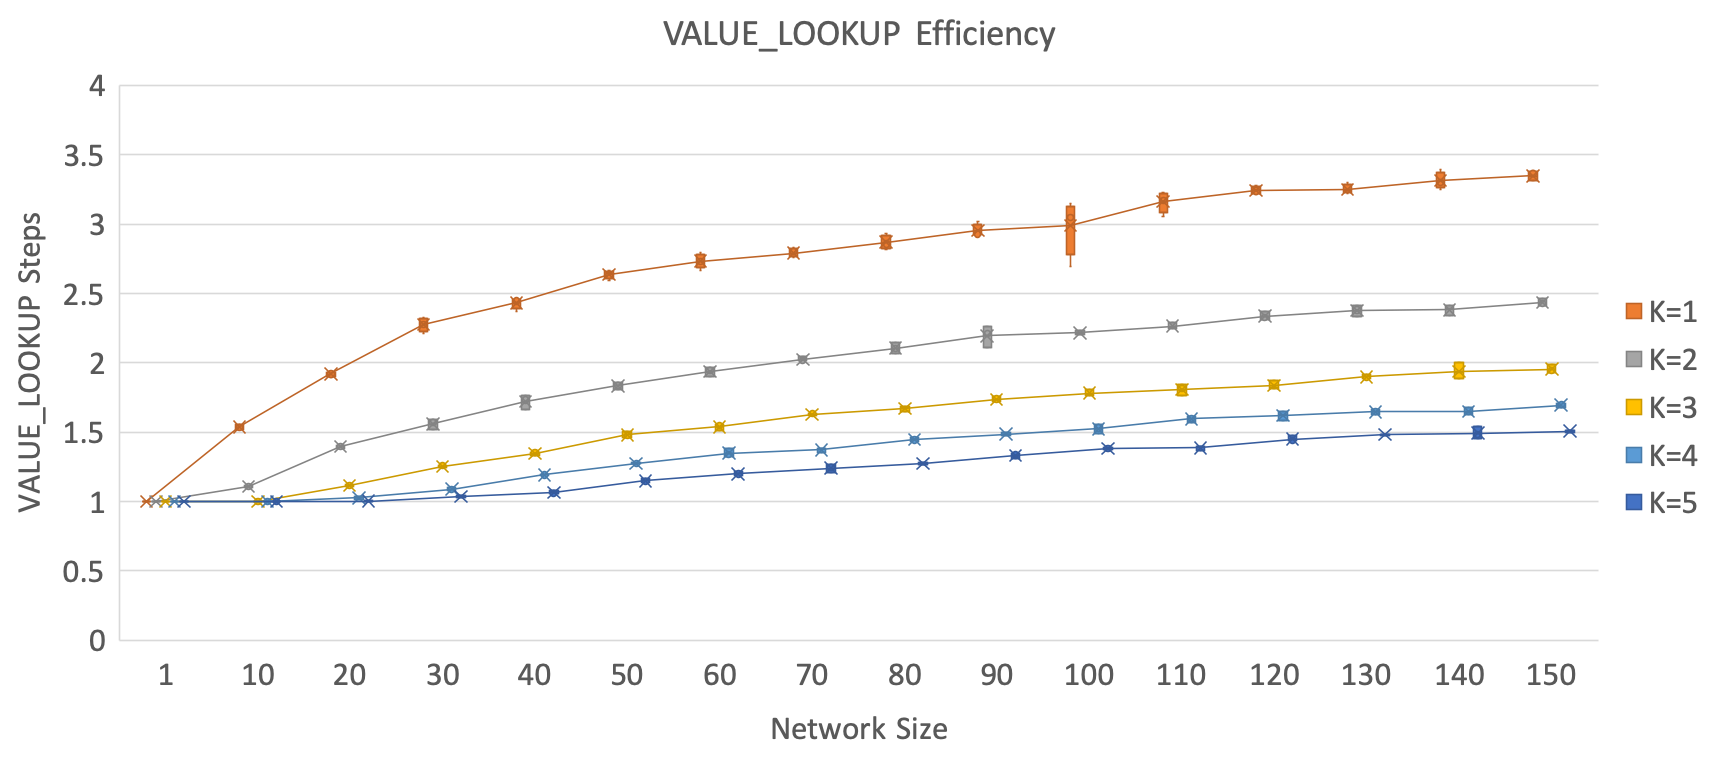
\includegraphics[width=14cm]{charts/chart_value_lookup_efficiency.png}
  \caption[VALUE\_LOOKUP steps with respect to $K$ and network size $n$]{VALUE\_LOOKUP steps with respect to redundancy parameter $K$ and network size $n$. Like \ref{fig:nodelookupefficiency}, VALUE\_LOOKUP steps also grows with network size following a logarithm curve, while number of steps needed is far less than that needed by NODE\_LOOKUP.}
  \label{fig:valuelookupefficiency}
\end{figure}

From figure \ref{fig:valuelookupefficiency}, we can observe that VALUE\_LOOKUP also follows a logarithm curve, but the number of steps needed is far less than that needed by NODE\_LOOKUP shown in \ref{fig:nodelookupefficiency}. In a FileFarm network of 100 farmers, it only takes less than 3 steps to find a shard. Besides, as $K$ increases, number of steps decreases roughly with a factor $H_{K}$ depicted by Cai\cite{cai2013probabilistic}. Putting this result with \ref{s:expnodelookupefficiency}, we can conclude that a larger choice of $K$ results in more uploading overhead, while improves downloading performance, as NODE\_LOOKUP and VALUE\_LOOKUP are needed before uploading / downloading a shard, respectively.

% exp: Retrievability
\section{Experiment: Retrievability}
\label{s:expretrievability}

Retrievability is one of the most important metrics used to measure quality of a cloud storage system. In this experiment, we want to examine how FileFarm is likely to hold client's data, and how certain configuration parameters affect the likelihood of uploaded files to be retrievable by clients. To be precise, we define retrievability as:

\begin{center}
  $Retrievability = \frac{\# Successfully Reconstructed}{\# Total Download Attempts}$
\end{center}

\noindent Belows are the configuration parameter to be considered in this experiment:

\begin{enumerate}
  \item $\alpha$: Online probability of each farmer.
  \item $K$: Number of redundant copies stored for each shard.
  \item $q$: Redundancy parameter in a (4, q) IDA schema; A file is recoverable given any 4 out of the (4+q) shards.
\end{enumerate}

As for the experimental procedure, we runs 20 farmers with online probability $\alpha$. After the farmers are bootstrapped, we run 500 clients and make them start random uploading/downloading. For each download request, the client reports if the file is successfully reconstructed. We Collect 10,000,000 reports from clients and compute retrievability. The whole process is repeated for $K=1,2,3$, $q=0,1,2$ and $\alpha=0.9,0.99,0.999,0.9999$.

\begin{table}[hbt]
  \centering
    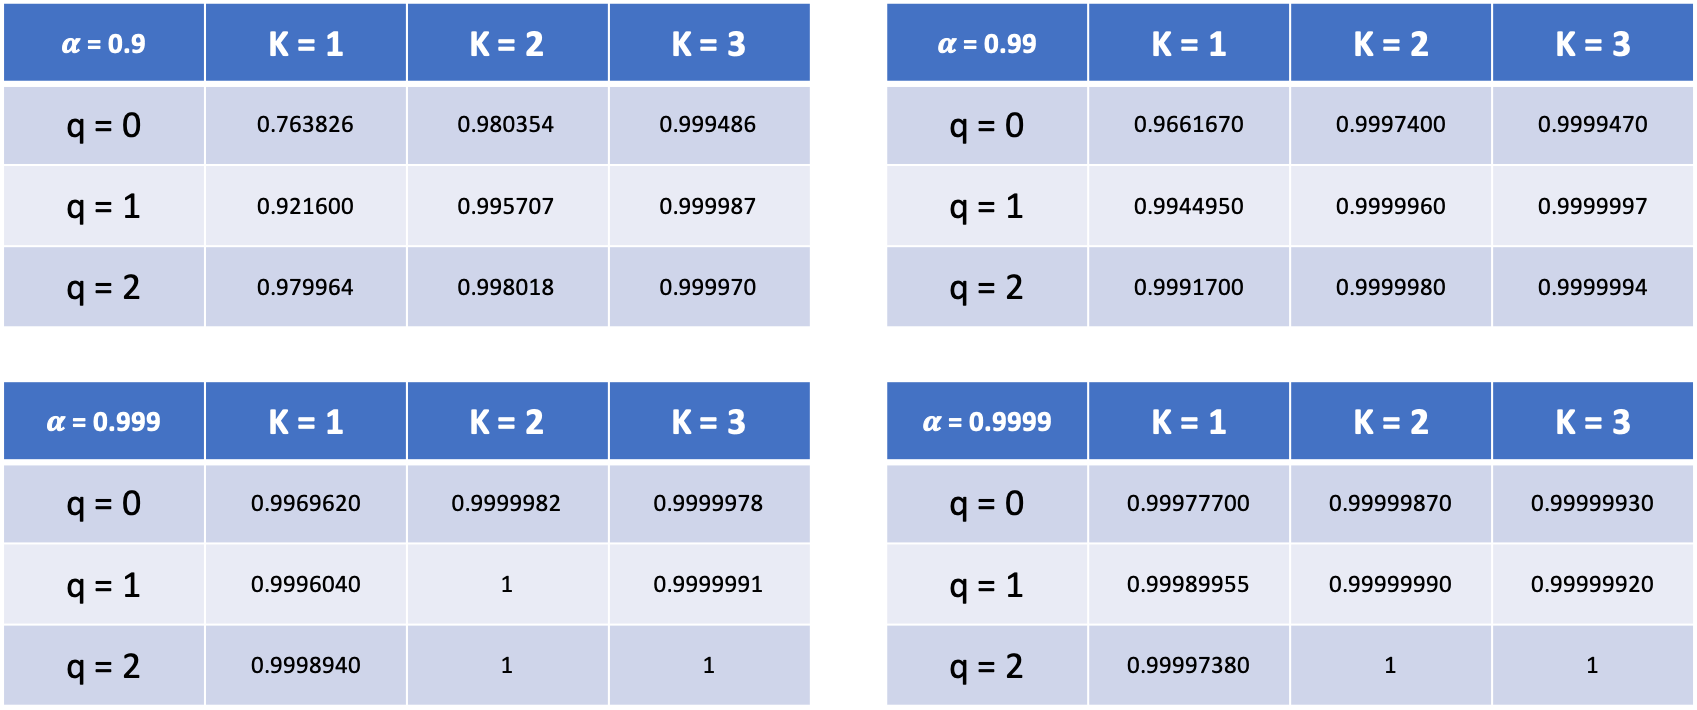
\includegraphics[width=14cm]{tables/table_retrievability.png}
    \caption[Retrievability of files with respect to farmer's online probability $\alpha$, network redundancy parameter $K$ and IDA redundancy parameter $q$]{Retrievability of files with respect to farmer's online probability $\alpha$, network redundancy parameter $K$ and IDA redundancy parameter $q$. The table shows that increasing $K$ and $q$ can both improve retrievability of files effectively.}
    \label{table:retrievability}
\end{table}
  
\begin{figure}[hbt]
  \centering
    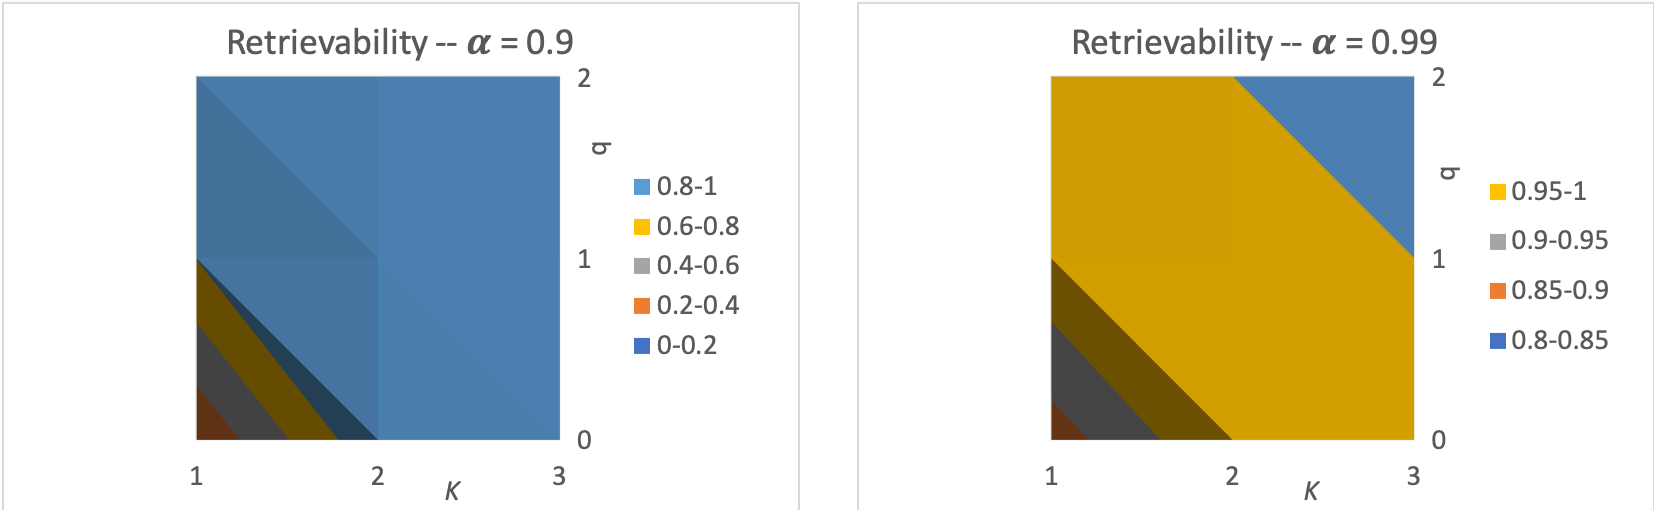
\includegraphics[width=14cm]{charts/chart_retrievability.png}
    \caption{Retrievability of files with respect to $\alpha$, $K$ and $q$}
    \label{fig:retrievability}
\end{figure}

From the result shown in \ref{table:retrievability}, we observe that network redundancy parameter $K$ and IDA redundancy parameter $q$ both effectively impact the retrievability of files. By increasing $K$, retrievability can be improved significantly. However, increasing $K$ has a relatively large overhead, considering the fact that an incremental in $K$ will consume an extra amount of storage space equaling to the actual file size. To reduce cost while preserving retrievability, increasing $q$ is a reasonable choice. In addition, we also observe that a selection of $K=2$ roughly squares the data lost probability. For example, within a system where farmers have $0.1$ probability to be offline (i.e. $\alpha=0.9$), a setting of $K=2 and q=1$ roughly achieves the data lost rate of $0.1^{2}=0.01$, which is effective considering the fact that a public cloud service normally has much lower probability to be unavailable, and we can make the probability of losing data even lower by building FileFarm upon them. Note that in some of the experimental cases where $\alpha>=0.999$, retrievability of files are estimated to be 1, which means we didn't observe any fail-to-download event in the 10,000,000 download attempts.

% exp: Throughput
\section{Experiment: Throughput}
\label{s:expthroughput}

In this experiment, we want to test FileFarm's I/O performance under different file size and sharding schemes. As described in figure \ref{fig:uploadflow} and figure \ref{fig:downloadflow}, the upload process of FileFarm involves slicing, encryption, IDA computation, NODE\_LOOKUP, ... while the download process involves VALUE\_LOOKUP, IDA computation, decryption, combining... Some of the operations can be done in parallel while others cannot. To analyze performance of such complicated flows, we run experiments, measure the elapsed time and compute throughput as follows:

\begin{center}
  $Throughput = \frac{File Size(MB)}{Elapsed Time(Sec)}$
\end{center}

As for the experimental procedure, we runs 5 farmers and 5 clients in total. Each farmer is assumed to have a 10 MB/s upload bandwidth. Once all farmers and clients are bootstrapped, we let clients start random upload and download files of size $S$ with a sharding scheme which generates $p$ shards in total. While uploading and downloading, we let clients report time consumption for each operations until 100 upload and 100 download reports have been collected. We collect these reports and compute mean of upload/download throughput. The whole process is repeated for $S=1,4,16,64,256,1024$ and $p=1,2,4,8,16,32$.

\begin{figure}[hbt]
\centering
  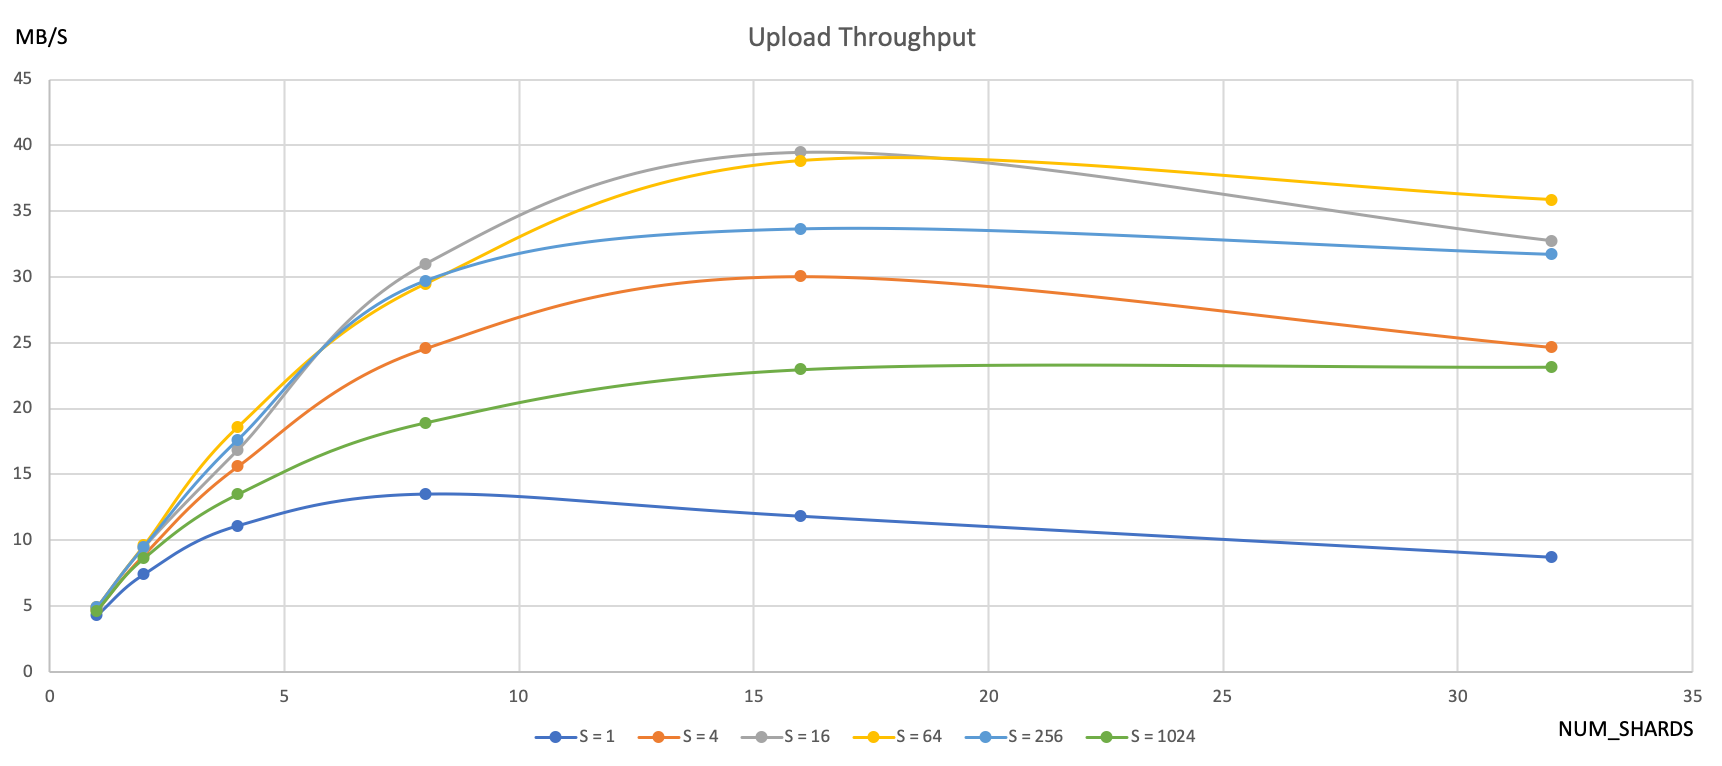
\includegraphics[width=14cm]{charts/chart_upload_throughput.png}
  \caption[Upload throughput with respect to file size and number of shards]{Upload throughput(MB/s) with respect to file size(MB) and number of shards $p$. With a file of size 64 MB, a sharding schema in which $p=16$ brings a best performance of around 39 MB/s.}
  \label{fig:uploadthroughput}
\end{figure}

\begin{figure}[hbt]
\centering
  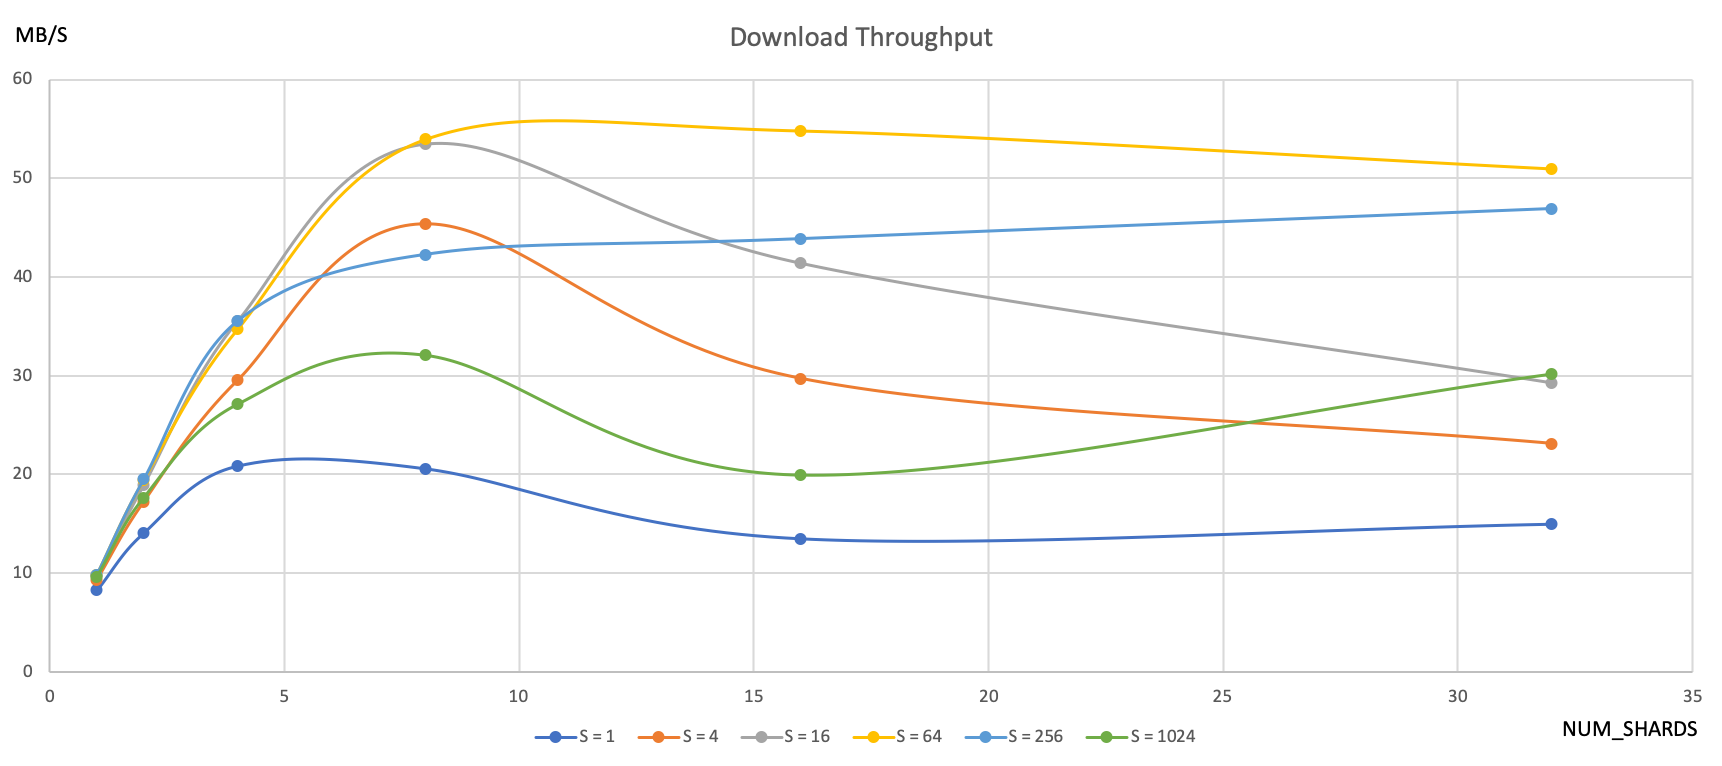
\includegraphics[width=14cm]{charts/chart_download_throughput.png}
  \caption[Download throughput with respect to file size and number of shards]{Download throughput(MB/s) with respect to file size(MB) and number of shards $p$. With a file of size 64 MB, a sharding schema in which $p=8$ brings a best performance of around 54 MB/s.}
  \label{fig:downloadthroughput}
\end{figure}

From the result shown in figure \ref{fig:uploadthroughput}, we observe that uploading throughput grows when number of shards increases. This is due to the system design in which shards are uploaded in parallel. This growing trend achieves saturation when number of shards $\approx 16$, where in-coming throughput of farmers achieves the NIC capacity limit of 10 Gbit/s. In the cases of smaller file size ($S$ = 1MB or 4MB), the curve goes down slightly with number of shards $> 16$. This is caused by the preprocessing cost of NODE\_LOOKUP, slicing, encryption, hashing, and IDA computation. When file size is relatively small, the preprocessing cost takes a significant term of timing overhead, while in cases of larger file size, the curve is mainly limited by farmers' NIC capacity.

Observing from chart \ref{fig:downloadthroughput}, we discover that download throughput roughly shares the same trends as upload throughput in terms of sharding schema and file size. However, there is a noticeable difference: download throughput is much higher than upload throughput. This is because of the fact that download only involves retrieval of 1 copy of the shard instead of $K$; thus, download operations induce less inter-farmer traffic than upload ones. In our experimental settings, number of physical hosts and NIC capacity on each host are limited and are easily stuffed by frequent client requests. Thus, inter-farmer traffic is easily bounded by hardware limitations and affect I/O performance. In real-world applications, however, the throughput bottleneck often occurs at client-side instead of farmer-side. Thus, upload/download throughput will mainly be determined by client bandwidth.

% exp: Cost -- Storage Release
\section{Experiment: Cost -- Storage Release}
\label{s:expcoststoragerelease}

The purpose of this experiment is to evaluate the cost-down effectiveness of \textit{storage release} mechanism. By description in \ref{ss:storagerelease}, storage release is a cost-reducing mechanism addressing redundant \textit{static storage fee}, which comes up with scenarios of service outage or migration of storage providers. To investigate the effect of storage release, we simulate a migration scenario. The experimental procedure goes as follows: we first start a network of 3 public farmers and 50 clients. Clients are allowed to randomly upload files until a total of 2,000 files are stored in the network. After the 2,000 files are stored in the network of 3 public farmers, we bootstrap another public farmer and let it join the network. Due to the \textit{key republishing} mechanism of Kademlia, some of the shards will start to be replicated to the newly-joined farmer. We then record the total static storage fee every simulational month until a year passed. We run this whole procedure in 3 different settings: (1) migration with storage release, (2) migration without storage release, (3) no migration and plot the growing curve of total static fee charged by public storage providers.

\begin{figure}[hbt]
  \centering
    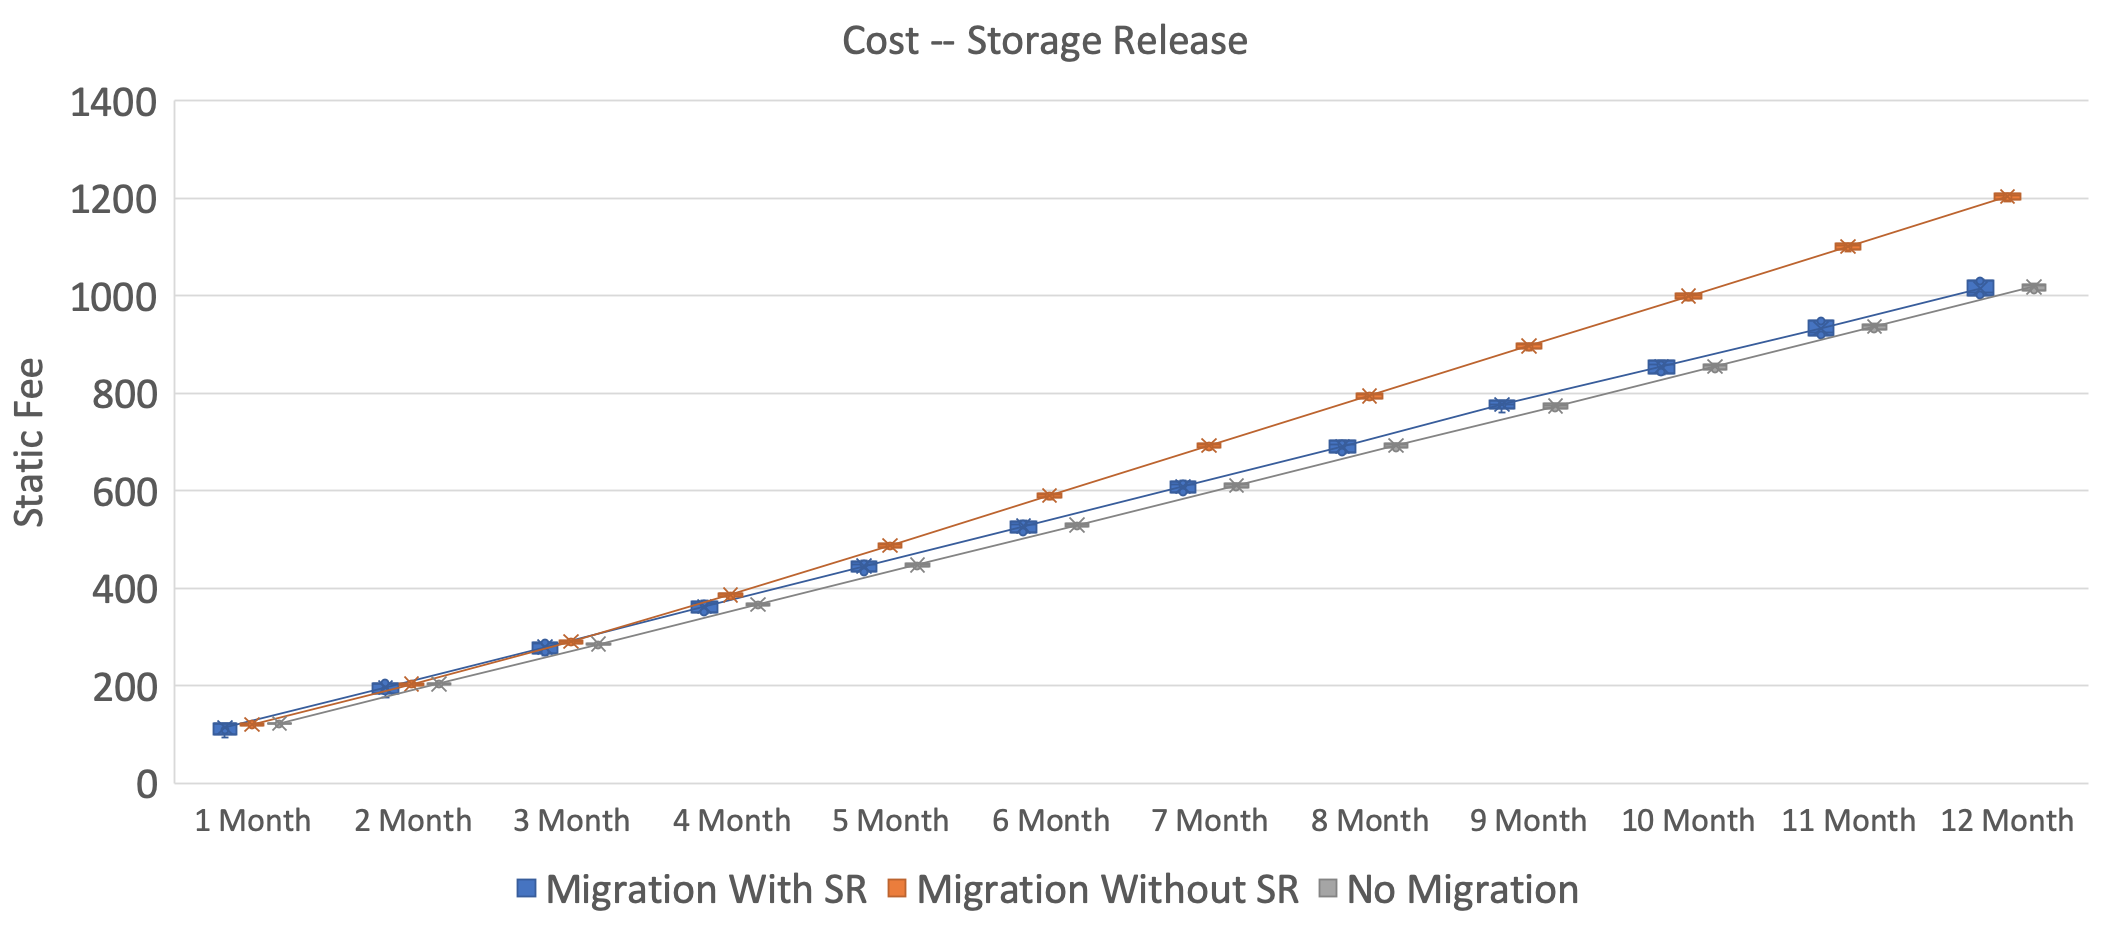
\includegraphics[width=14cm]{charts/chart_cost_storage_release.png}
    \caption[Growth curve of static fee in 3 different settings: (1) migration with storage release, (2) migration without storage release, (3) no migration]{Growth curve of static fee in 3 different settings: (1) migration with storage release, (2) migration without storage release, (3) no migration. By enabling storage release, a 21.1\% of storage cost overhead is avoided, with the cost curve sticking to that of non-migration case.}
    \label{fig:coststoragerelease}
\end{figure}

From figure \ref{fig:coststoragerelease}, we can observe that static storage fee grows linearly with time. This is due to our experimental settings that a fixed number of files are stored on the network after migration occurs, and thus monthly fees are charged according to the size of static files. Besides, we can also observe that in the case of \textit{migration without storage release}, the cost trend is steeper then that of other 2 cases, which implies that a static number of redundant shards are stored on public clouds. These redundant shards then induces a fixed cost every month. In the context of this experiment where number of farmers migrates from 3 to 4, the storage overhead is roughly $21.1\%$ more than the case where no migration occurs. By enabling storage release, this overhead can be avoided, with the cost curve sticking to that of non-migration case.

% exp: Cost -- Prioritized Download
\section{Experiment: Cost -- Prioritized Download}
\label{s:expcostprioritizeddownload}

In this experiment, we want to evaluate the cost preserved by the \textit{prioritized download} mechanism in a hybrid setting where both public clouds and private servers contribute to the storage network, while public clouds charge storage fees but private servers do not. As described in \ref{ss:prioritizeddownload}, the prioritized download mechanism saves \textit{data transfer out} fee by settings preference to downloading from private farmers over public ones. Thus, we conduct experiment according to such hybrid scenario: we first bootstrap 25 farmers, with $N$ of them public farmers and other $(25-N)$ of them private ones.  Then we start 50 clients and let them upload and download files randomly. We record the transfer fee accumulated in the following 3 minutes and compare the total fee in 2 cases: (1) with prioritized download, (2) without prioritized download. The whole procedure is repeated for $N = 1, 2, 4$.

\begin{figure}[hbt]
  \centering
    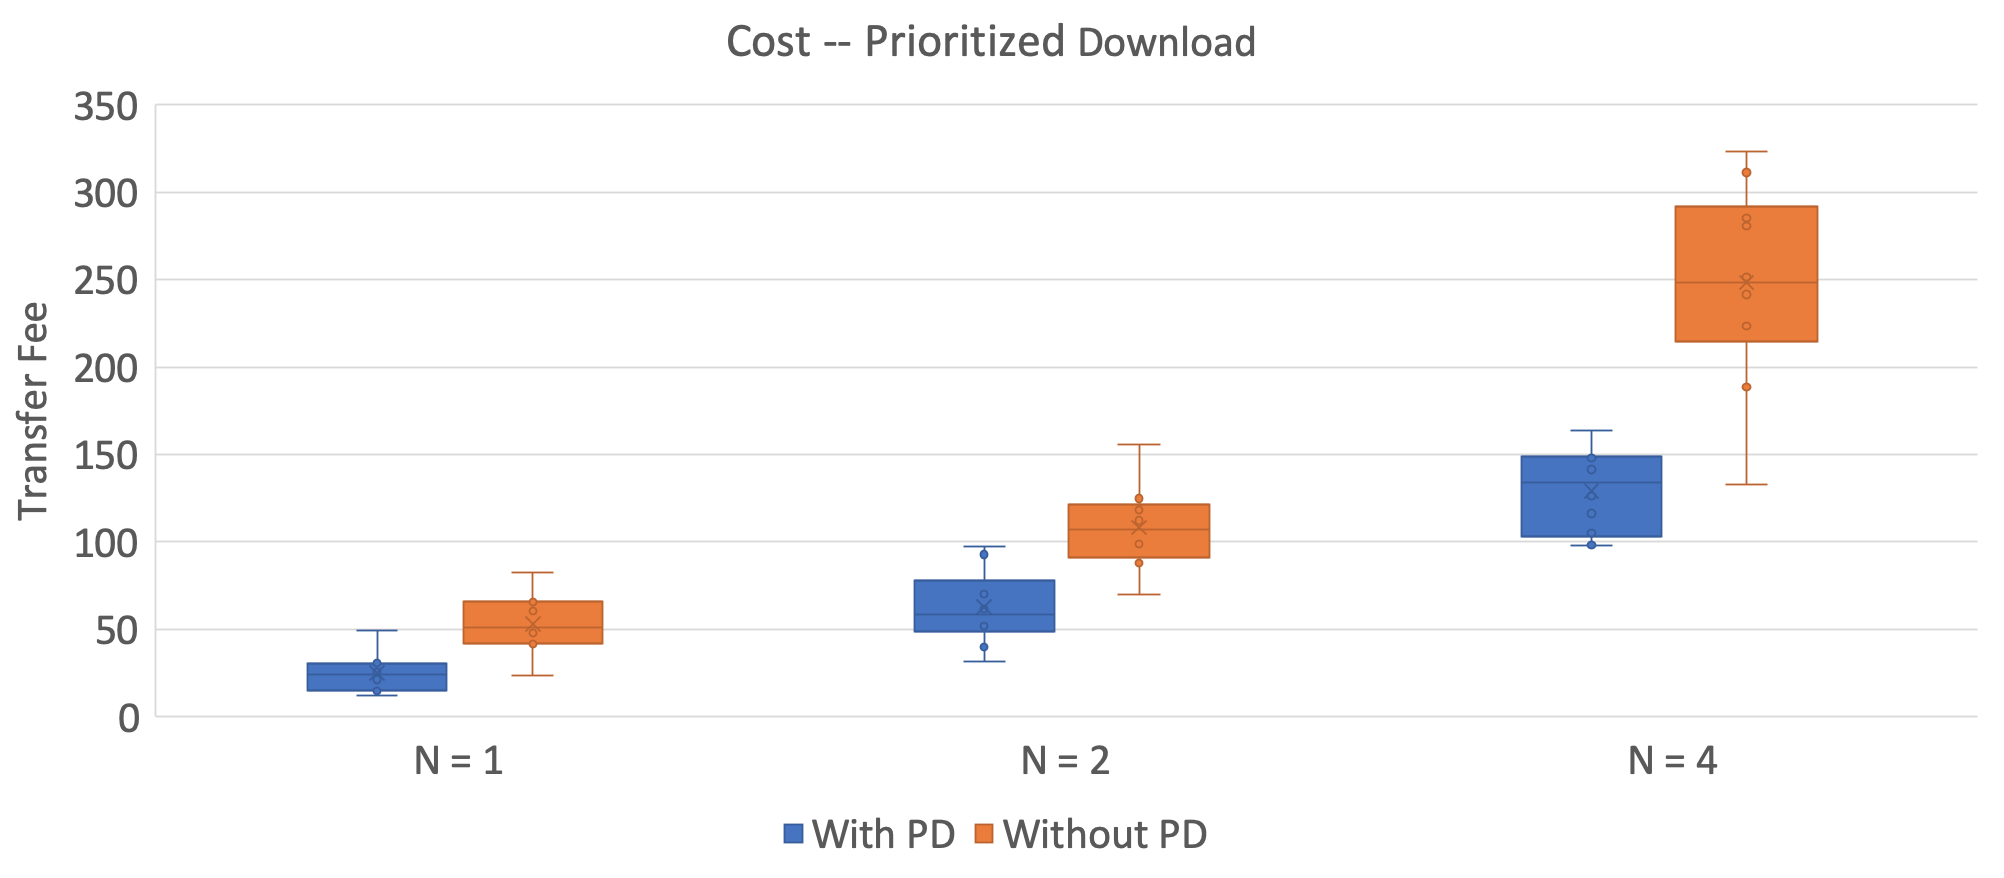
\includegraphics[width=14cm]{charts/chart_cost_prioritized_download.png}
    \caption[Comparison of transfer fee in 2 cases: (1) with prioritized download, (2) without prioritized download]{Comparison of transfer fee in 2 cases: (1) with prioritized download, (2) without prioritized download. Prioritized download mechanism preserves 47.6\% of transfer fee in average}
    \label{fig:costprioritizeddownload}
\end{figure}

From figure \ref{fig:costprioritizeddownload}, we observed that prioritized download saves 52.3\%, 42.0\%, 48.0\% of \textit{data transfer out fee} in the cases of $N = 1, 2, 4$, respectively. Since \textit{prioritized download} only changes the preference of downloading order, this saving of cost only applies to \textit{data transfer out fee} but not \textit{static fee}. With the same sense, \textit{prioritized download} has no impact on retrievability of files since shards are still saved and available on the public clouds, only with lower access rates.



  